
\documentclass[12pt, oneside]{amsart}
\usepackage[font={sf}]{caption}
\usepackage[]{graphics}
\usepackage{graphicx}
\usepackage{epstopdf}
\usepackage{hyperref}
\hypersetup{breaklinks=true, colorlinks=true, citecolor=blue}
\usepackage{natbib}
\usepackage{color}
\usepackage{soul}
\usepackage{rotating}
\usepackage{tabularx}
\usepackage{longtable}
\usepackage{lscape}
\usepackage{array}
\usepackage{multirow}
\usepackage{setspace}
\usepackage{textcomp}
\usepackage{dcolumn}
\setlength{\LTcapwidth}{6in}
\usepackage{dcolumn}
\usepackage[margin=1in]{geometry}

 \bibpunct{(}{)}{,}{a}{}{,}
 \doublespacing
 \raggedright
 \setlength{\parindent}{15pt} 


\begin{document}
%\setcounter{secnumdepth}{0}


{ \Large \bf Supplementary Figures}

Lotterhos et al. 2017. (Add Title Here). Methods in Ecology and Evolution.

\hspace{3cm}

%\tableofcontents
%\listoftables
%\renewcommand\thesection{S1}
%\listoffigures

\renewcommand{\figurename}{Supplementary Figure}

\begin{figure}[h]
\begin{center}
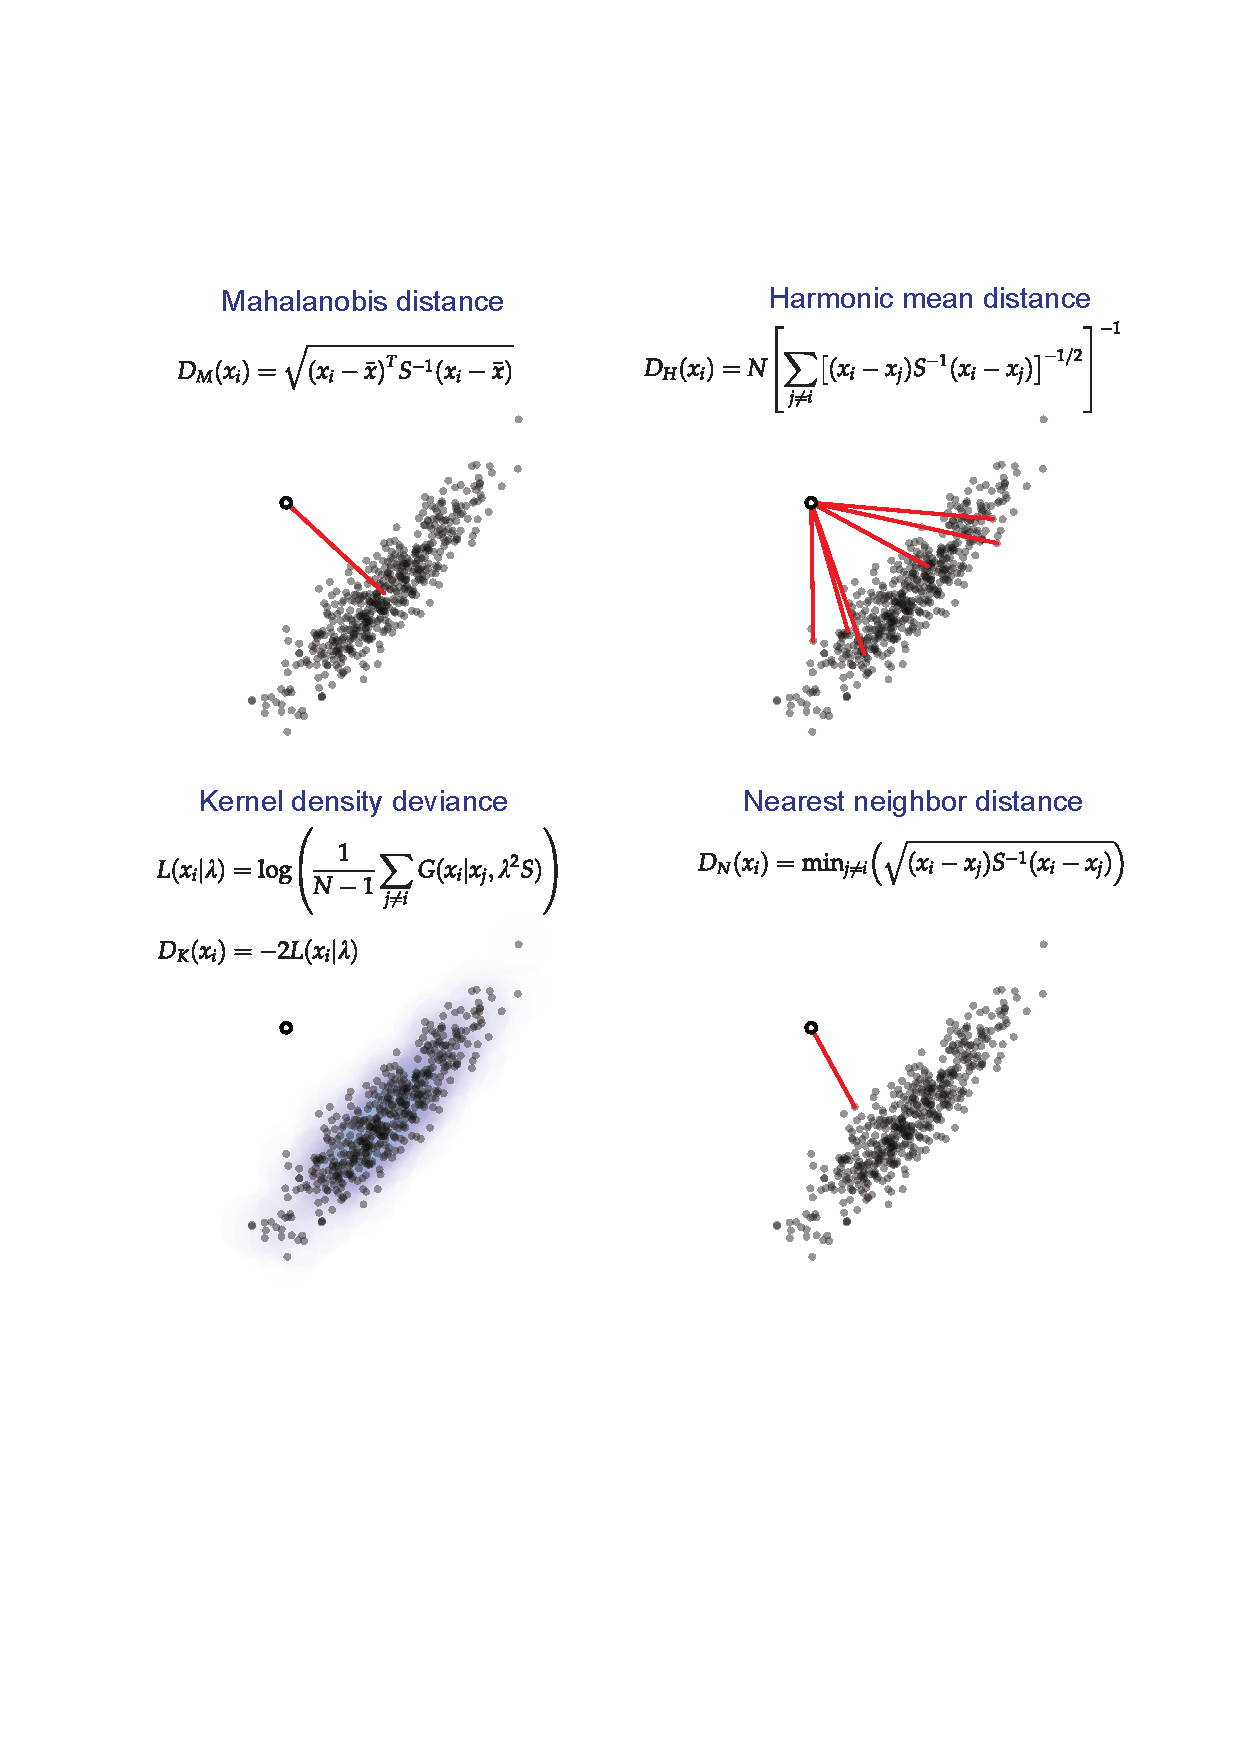
\includegraphics[width=6in]{../figures_man2/S1-bivariate.pdf}
\end{center}
\caption[]{Conceptual examples of the multivariate distance measures described in Verity et al. 2017  compared in this study (kernel density deviance was not included due to slow run times).}
 \label{fig:???}
\end{figure}

\begin{figure}[h]
\begin{center}
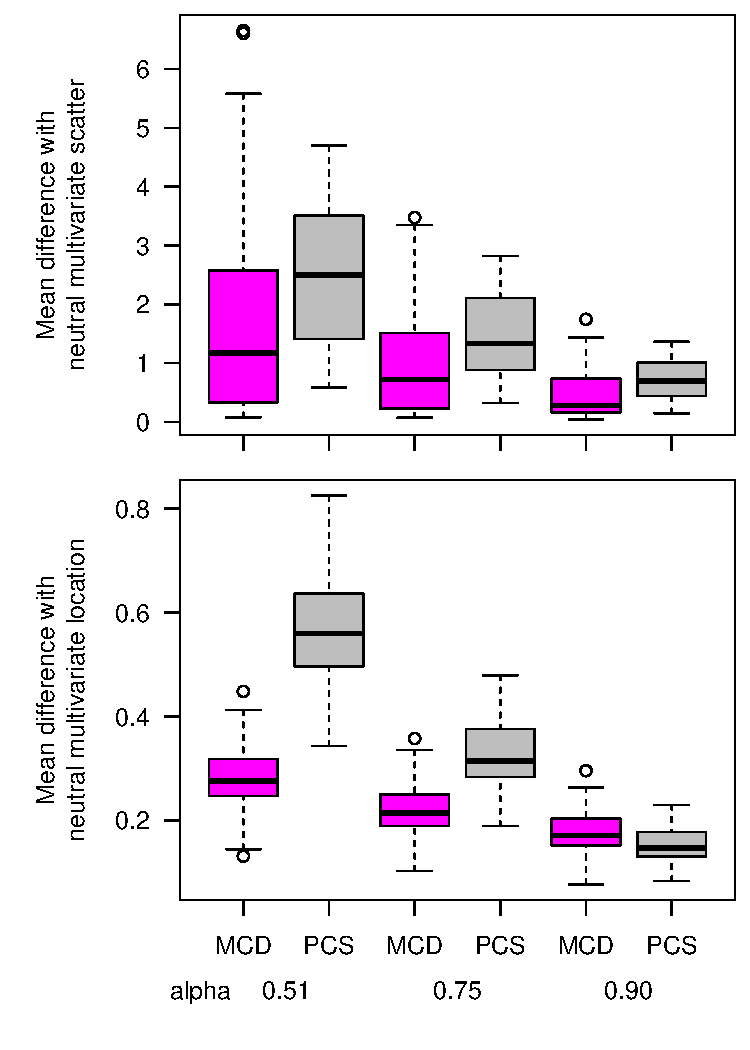
\includegraphics[width=4in]{../figures_man2/S2-LandsharcComparetoNeutlocationscatterPCSvsMCD.pdf}
\end{center}
\caption[]{Difference between the multivariate location and scatter estimated by the robust method and the true neutral estimate. MCD: minimum covariance determinant; PCS: projection congruent subset.
} 
 \label{fig:???}
\end{figure}



\newpage
\begin{figure}[h]
\begin{center}
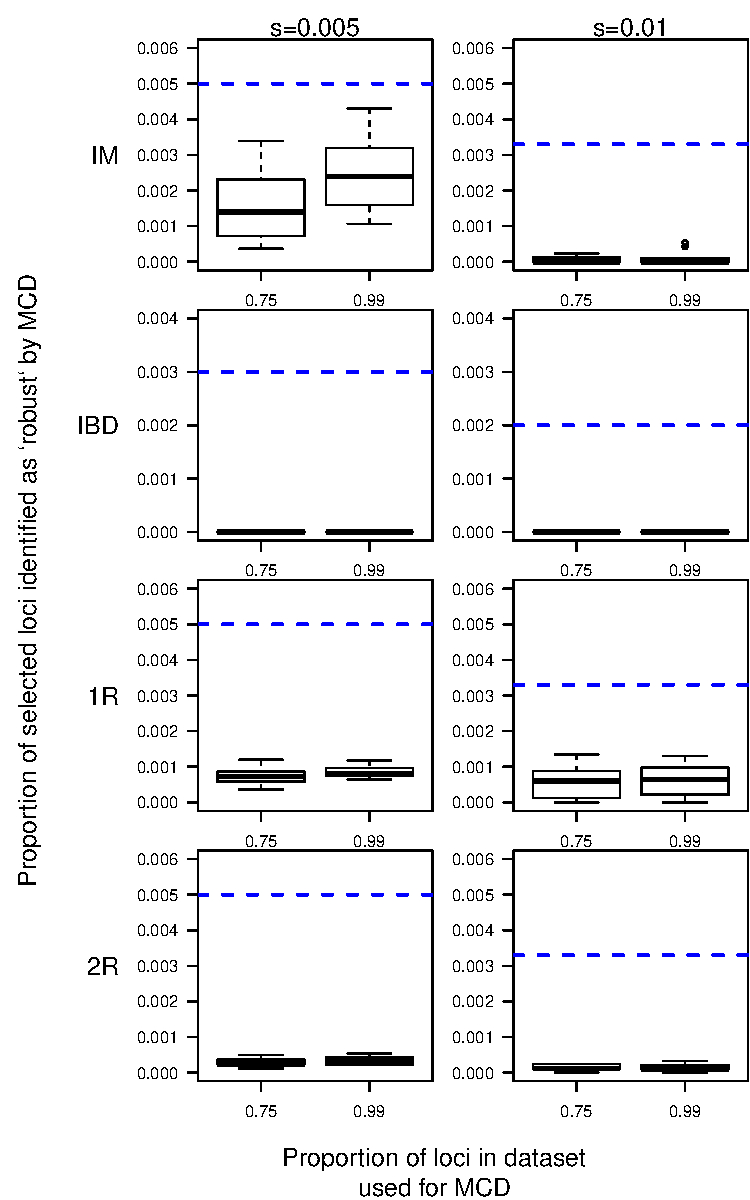
\includegraphics[height=6in]{../figures_man2/S3-LandsharcProportionSelectedMCD.pdf}
\end{center}
\caption[]{Evaluation of whether loci affected by selection were identified as 'robust' points (e.g., not outliers) by the MCD algorithm. Loci under relatively weak selection (s=0.005) are in the left column, well loci under moderate selection are in the right column (s=0.01). The horizontal dashed line represents the null expectation, based on the proportion of loci under that strength of selection in the entire dataset. The MCD never identified loci simulated under strong selection (s=0.1) as robust (expected = 0.001 in IBD and 0.0017 in IM, 1R, and 2R; observed = 0 across all simulations).} 
 \label{fig:???}
\end{figure}

\newpage
\begin{figure}[h]
\begin{center}
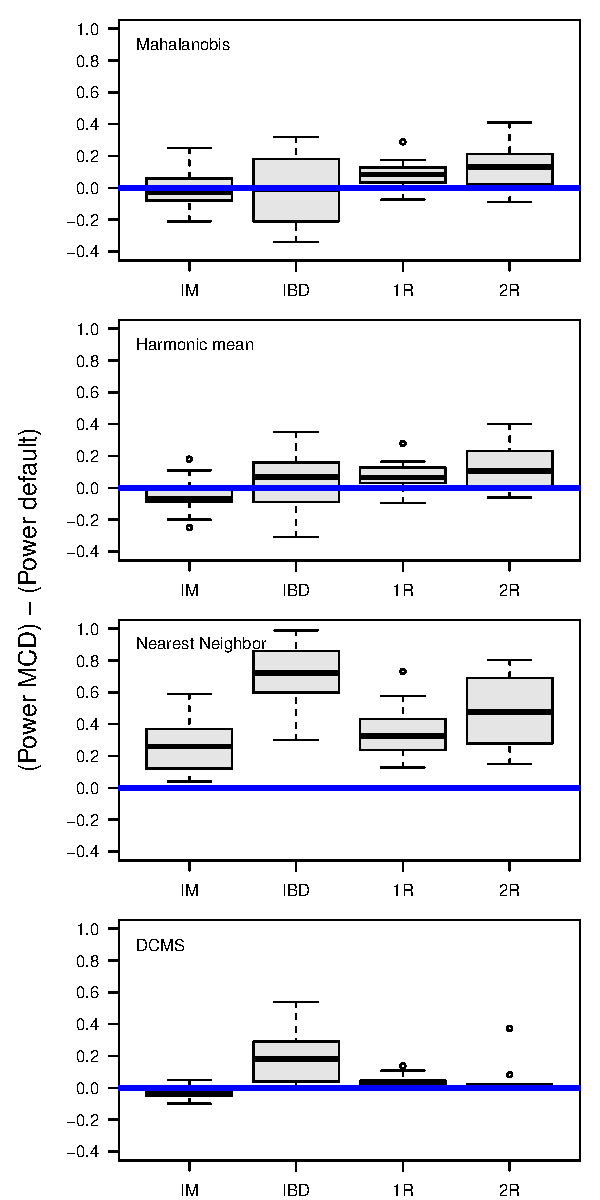
\includegraphics[width=4in]{../figures_man2/S4-LandsharcComparePowerMCDminusPowerDefaultByDemog.pdf}
\end{center}
\caption[]{The difference in empirical power of the statistic to detect selection with and without the robust points identified by minimum covariance determinant (MCD) used in the calculation for the four demographies: island model (IM), isolation by distance (IBD), range expansion from one refuge (1R), range expansion from two refugia (2R). } 
 \label{fig:???}
\end{figure}

\newpage
\begin{figure}[h]
\begin{center}
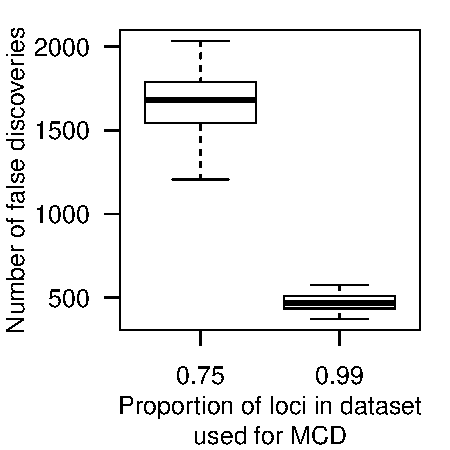
\includegraphics[width=4in]{../figures_man2/S5-LandsharcFalsePositivesMCD.pdf}
\end{center}
\caption[]{The number of false discoveries (neutral loci inferred to be outliers, out of 9900 total neutral loci in the dataset) resulting if robust points identified by the MCD are used as an empirical null distribution.} 
 \label{fig:???}
\end{figure}

\newpage
\begin{figure}[h]
\begin{center}
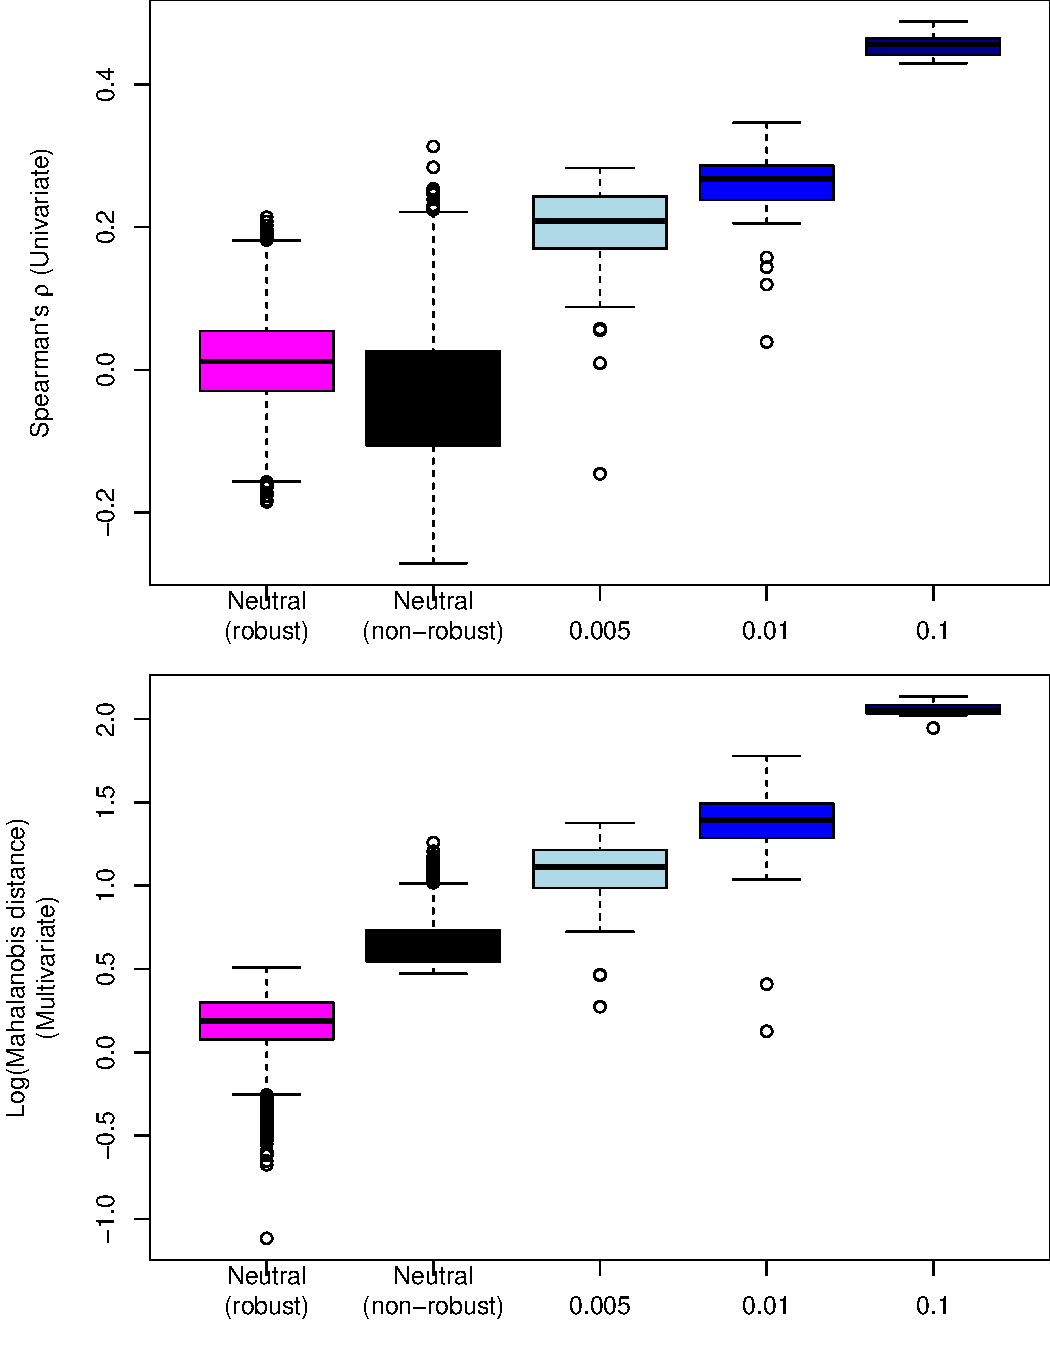
\includegraphics[width=6in]{../figures_man2/S6-LandsharcAverageSignals.pdf}
\end{center}
\caption[]{Average signals as a function of type of locus for a univariate statistic (top) and a multivariate distance (bottom).}
 \label{fig:???}
\end{figure}

\newpage
\begin{figure}[h]
\begin{center}
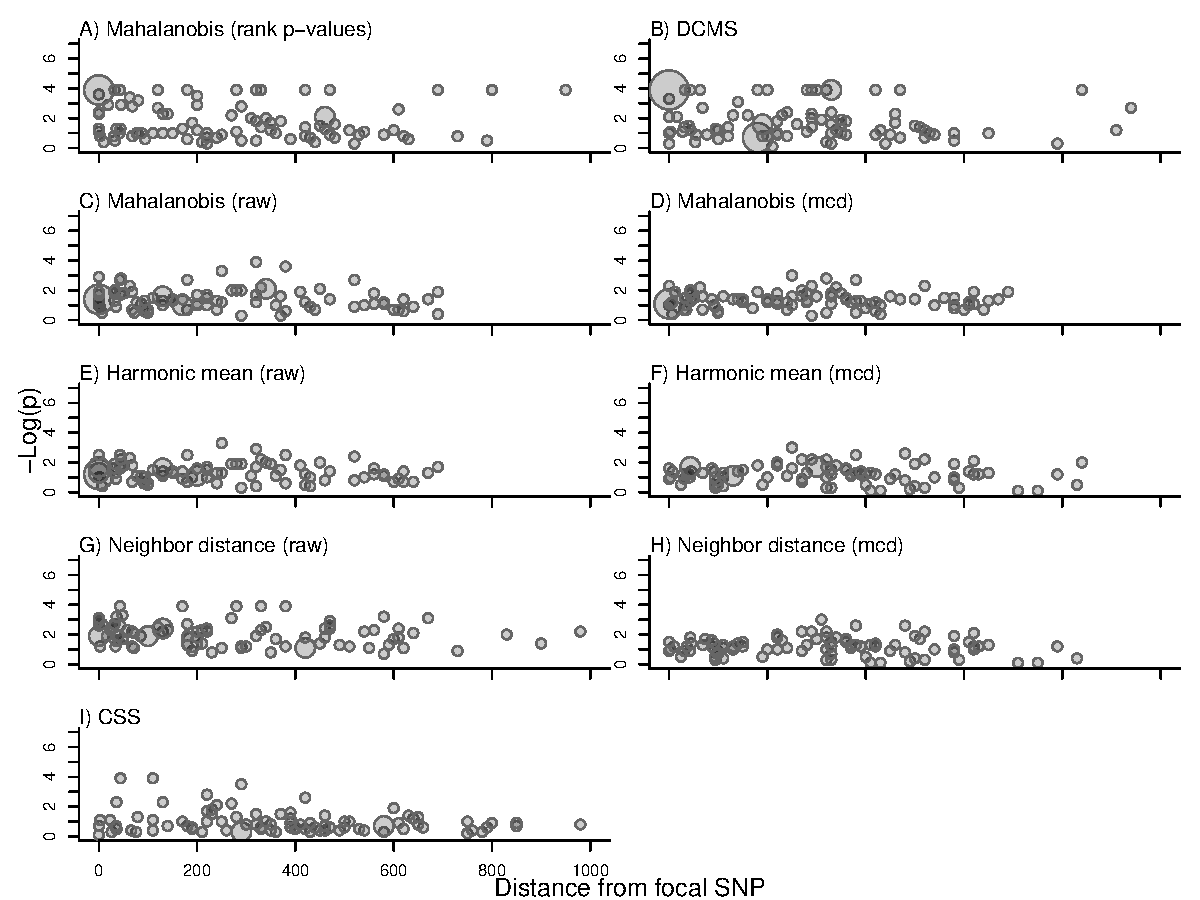
\includegraphics[width=6in]{../figures_man2/S7-Dog_ScatterCompareDistanceAndEmp_AllMulti.pdf}
\end{center}
\caption[]{Comparison among the compound measures for distance in the maximum of signal from the focal SNP versus the significance of the maximum signal, across all dog breeds and loci.. Upper left corner of the plot is higher performance.}
 \label{fig:???}
\end{figure}

\newpage
\begin{figure}[h]
\begin{center}
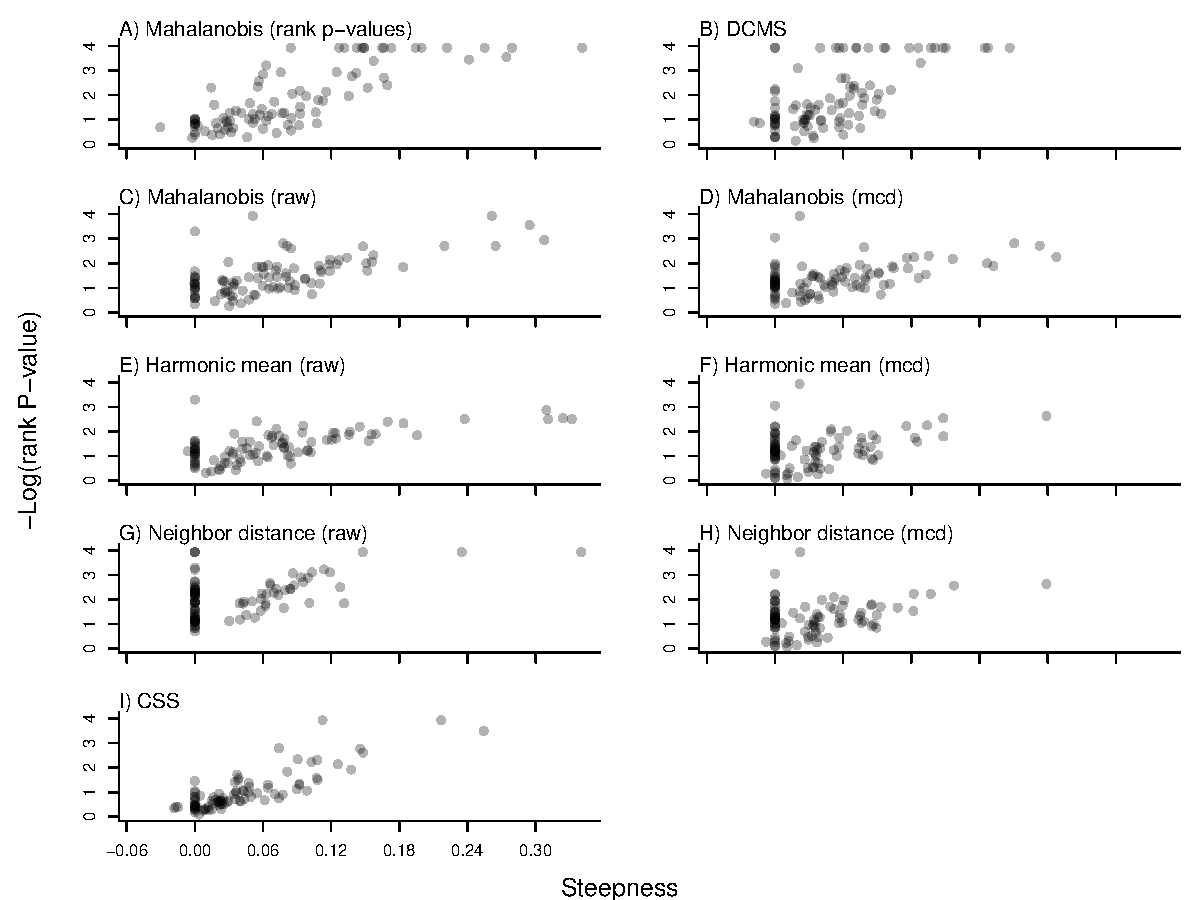
\includegraphics[width=6in]{../figures_man2/S8-Dog_ScatterCompareSteepnessAndEmp_AllMulti.pdf}
\end{center}
\caption[]{Comparison among the compound measures for steepness in the maximum of signal versus the significance of the maximum signal, across all dog breeds and loci.. Upper right corner of the plot is higher performance.}
 \label{fig:???}
\end{figure}

\newpage
\begin{figure}[h]
\begin{center}
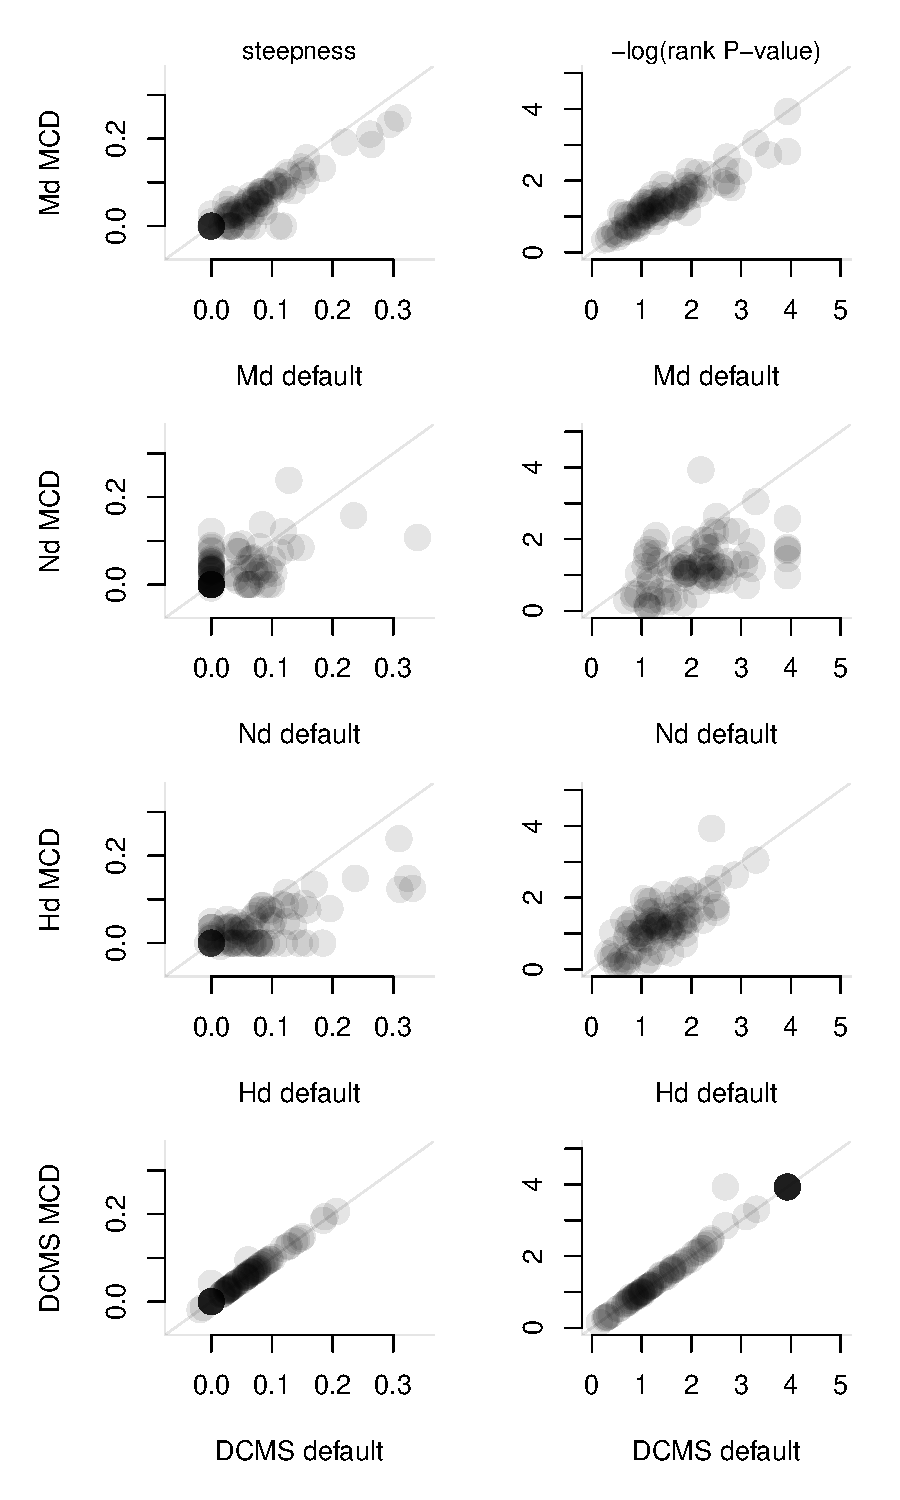
\includegraphics[height=6in]{../figures_man2/S9-Dog_scatterCompareDefaultMCD.pdf}
\end{center}
\caption[]{Comparison between any compound measure with versus without the MCD, for steepness in the left column and minus-log ranked $P$-value in the right column, across all dog breeds and loci.}
 \label{fig:???}
\end{figure}

\newpage
\begin{figure}[h]
\begin{center}
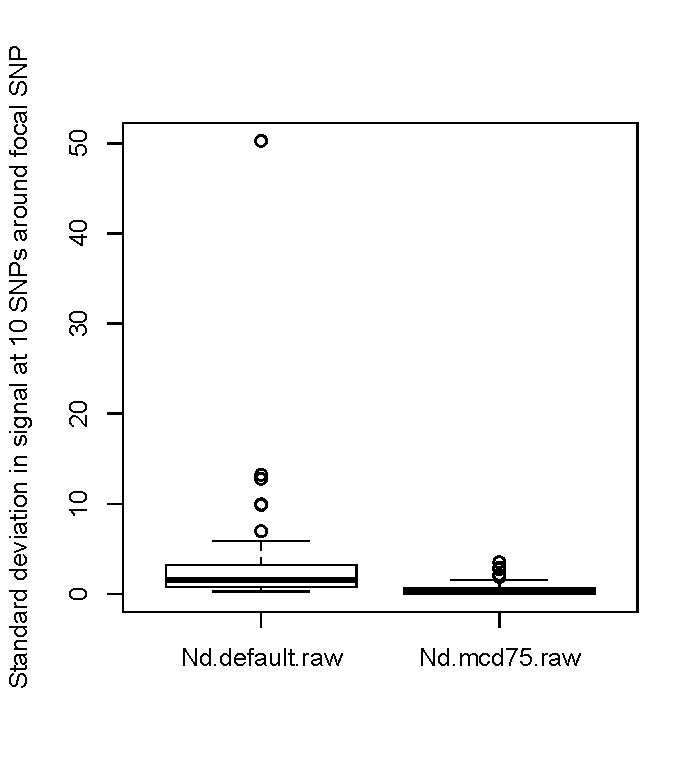
\includegraphics[width=6in]{../figures_man2/S10-Dog-CompareVarNd.pdf}
\end{center}
\caption[]{Boxplot showing standard deviation in the signal at 10 SNPs around the max SNP, across all dog breeds and loci. The default nearest-neighbor distance (Nd.default.raw) is compared to the Nd with the MCD (Nd.mcd75.raw), showing higher variance in the former because of spurious signals.}
 \label{fig:???}
\end{figure}

\newpage
\begin{figure}[h]
\begin{center}
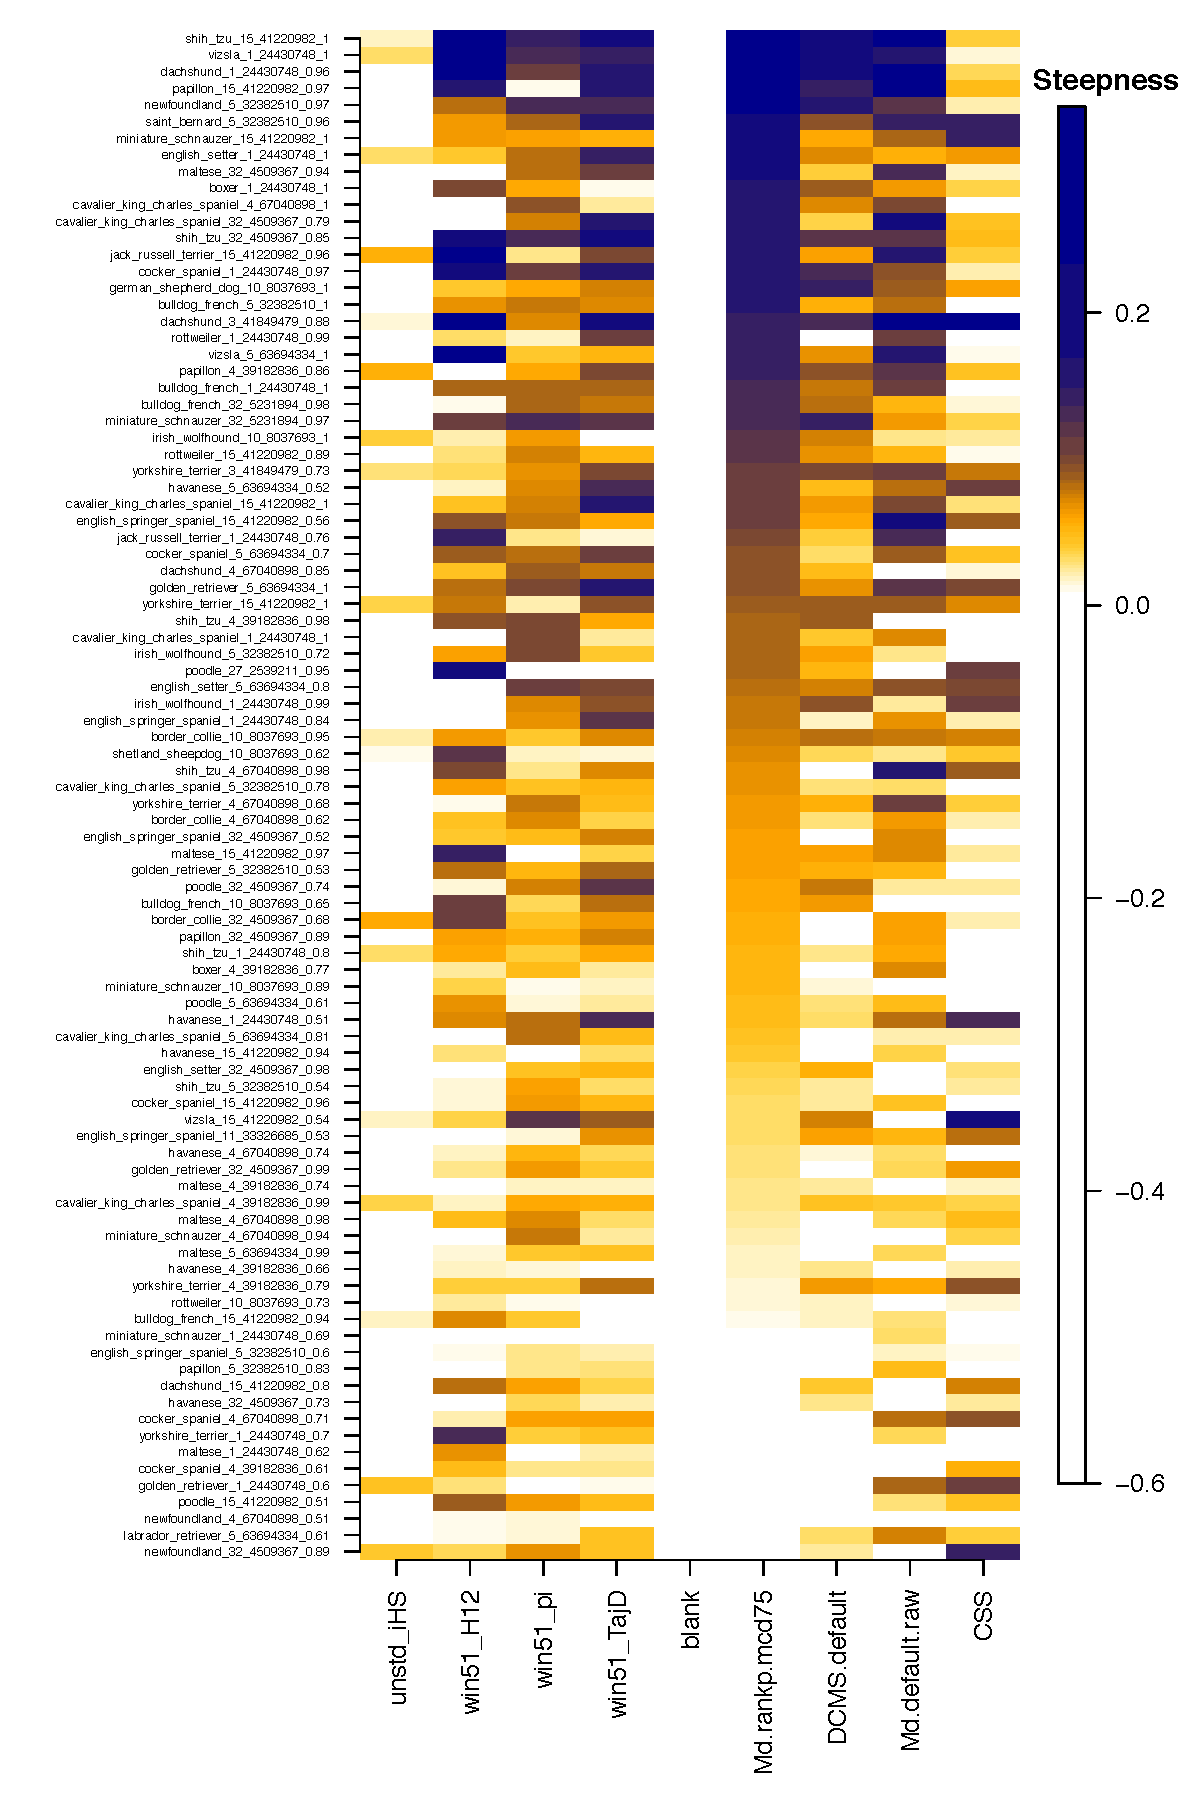
\includegraphics[height=6in]{../figures_man2/S11-Dog_heatmap_steepness_compare_stats.pdf}
\end{center}
\caption[]{Heatmap of steepness of the selection signal evaluated for each individual locus in the empirical dog dataset. Zero or negative values of steepness indicate the signal is absent or in the wrong direction.
The univariate statistics include iHS, H12, nucleotide diversity $\pi$, and Tajima's $D$. The compound measures include: the Mahalanobis distance based on minus-log fractional $P$-values (Md-rank-$P$), the decorrelated composite of multiple signals (DCMS), the Mahalanobis distance based on the raw statistics, and the composite signal of selection (CSS). The row labels indicate the dog breed, chromosome, base pair of the focal SNP, and the allele frequency of the focal SNP.

TO DO: EDIT X-AXIS LABELS}
 \label{fig:???}
\end{figure}

\newpage
\begin{figure}[h]
\begin{center}
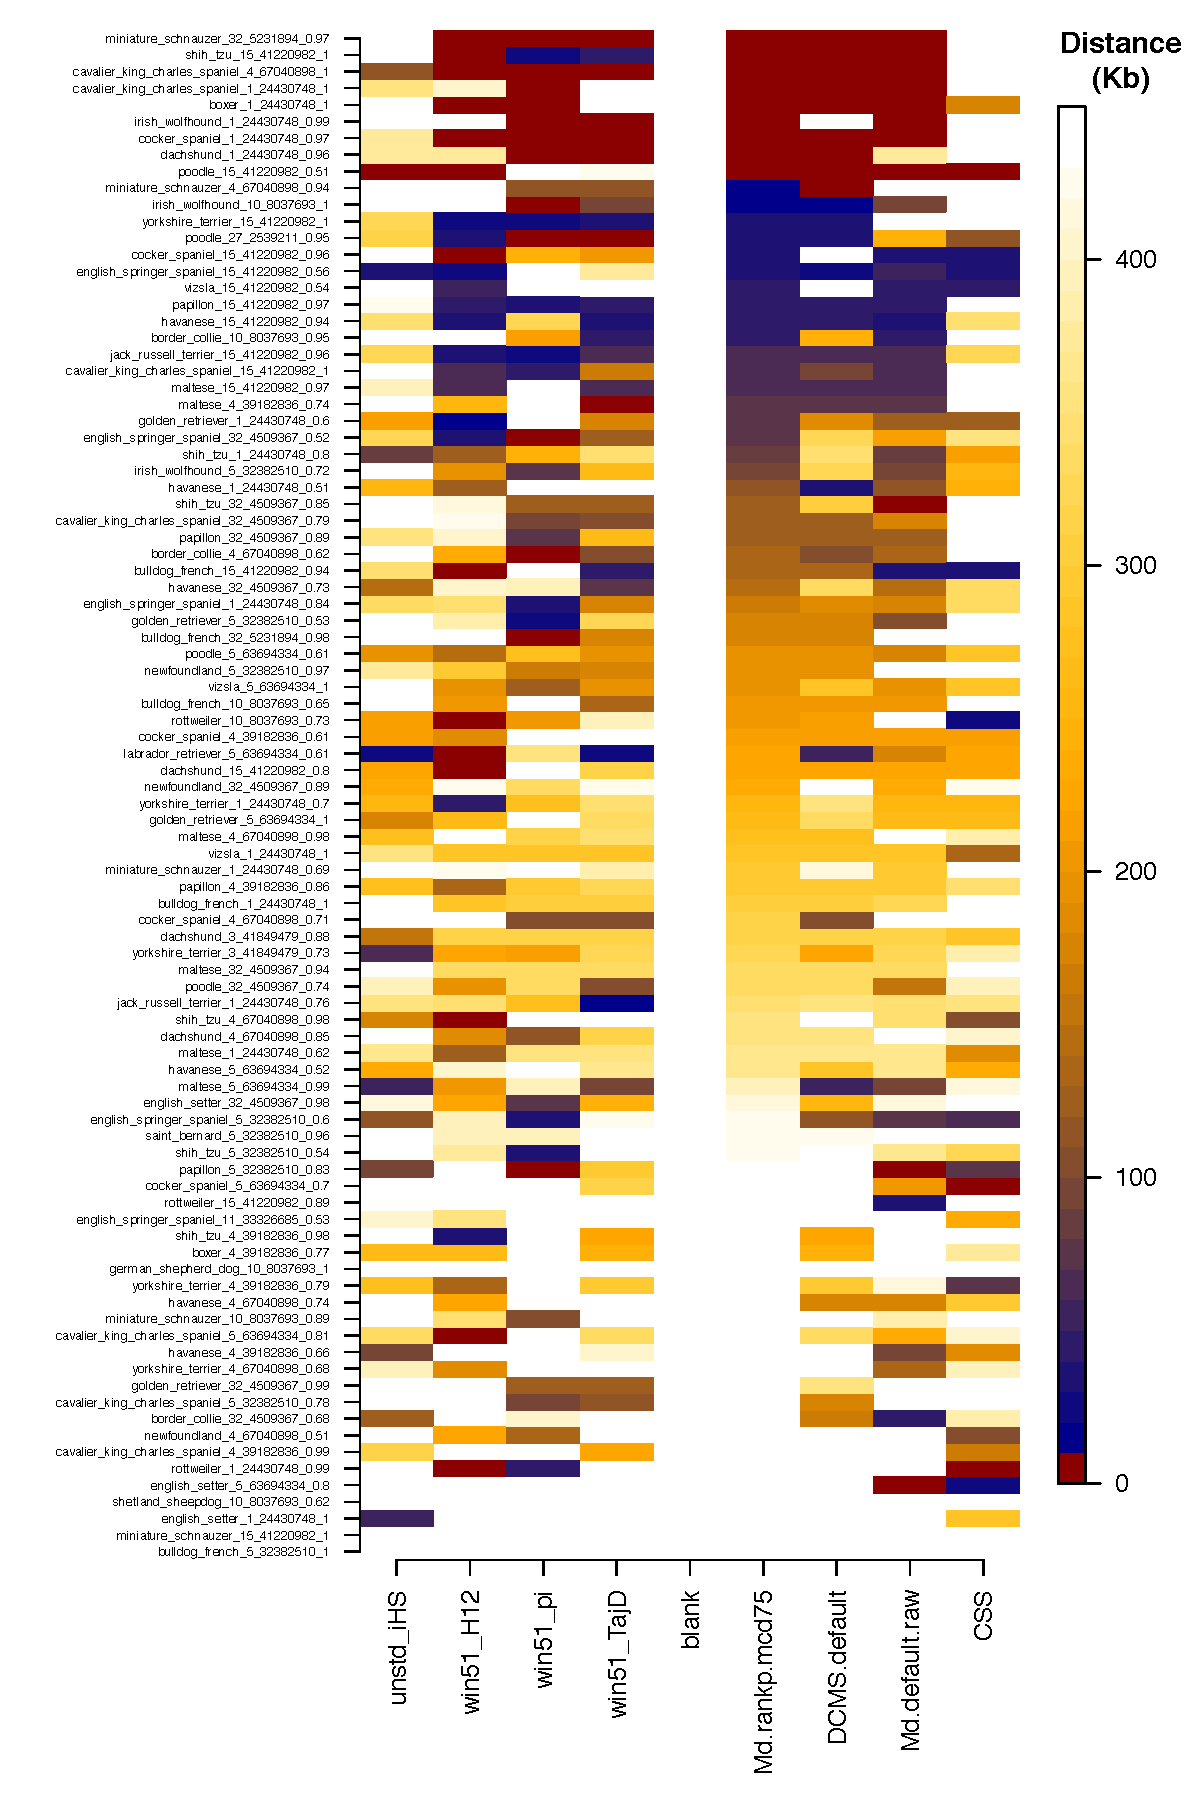
\includegraphics[height=6in]{../figures_man2/S12-Dog_heatmap_DIST_compare_stats.pdf}
\end{center}
\caption[]{Heatmap of distance in kilobases of the selection signal (max SNP) from the focal SNP, evaluated for each individual locus in the empirical dog dataset. Cases in which the focal SNP was genotyped and the maximum signal in the window was at this SNP (i.e., distance = 0) are colored dark red.
The univariate statistics include iHS, H12, nucleotide diversity $\pi$, and Tajima's $D$. The compound measures include: the Mahalanobis distance based on minus-log fractional $P$-values (Md-rank-$P$), the decorrelated composite of multiple signals (DCMS), the Mahalanobis distance based on the raw statistics, and the composite signal of selection (CSS). The row labels indicate the dog breed, chromosome, base pair of the focal SNP, and the allele frequency of the focal SNP.

TO DO: EDIT X-AXIS LABELS}
 \label{fig:???}
\end{figure}

\newpage
\begin{figure}[h]
\begin{center}
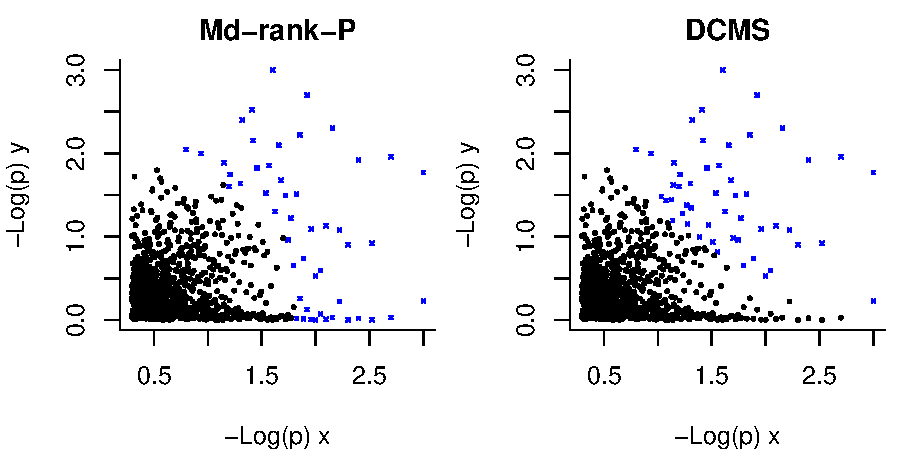
\includegraphics[width=6in]{../figures_man2/S13-CompareMdRankPandDCMS.pdf}
\end{center}
\caption[]{Comparison of Md-rank-P and DCMS on P-values obtained from a bivariate normal distribution. Black circles indicate points less than the 0.95\% of the compound measure and blue crosses indicate points above this threshold. In this toy example, some points are significant by both the $x$ and $y$ variables (points in upper right side of the graph), while other points are only significant by $x$ variable (lower right part of the graph).}
 \label{fig:???}
\end{figure}

\end{document}